\chapter{Desenvolvimento}
  \section{Requisitos}
  Para Sommerville requisitos de um sistema podem ser entendidos como sendo as descrições do que um sistema deve fazer, os sistemas que ele deve prover [SOMMERVILLE]. Estes requisitos refletem a necessidade do cliente para um sistema que serve a um propósito específico. Este conceito abrange não somente à requisitos de software mas a requisitos de produto também. Neste caso por não existir um cliente real, os requisitos foram levantados juntamente com os idealizadores do produto que são os próprios alunos. 
  Na tabela [REF TABELA] são elicitados os principais requisitos do produto "Bicicleta Elétrica com Dispositivo de Auxílio à Rota"
  
  
  
  \section{Software}
	\subsection{Aplicativo}
	
	\subsection{Comunicação APP e Microcontrolador}
	  A comunicação entre o celular e o microcontrolador será feita através de receptor \textit{bluetooth} acoplado ao microcontrolador. Para que seja feita essa comunicação, será utilizada a API do próprio sistema android para troca de informações via \textit{bluetooth}. Dentre os principais recursos que a API fornece, os que mais serão utilizados serão:
	  \begin{itemize}
	  	\item Busca por outros aparelhos \textit{bluetooth};
	  	\item Pareamento entre o adaptador \textit{bluetooth} e o dispositivo\textit{bluetooth};
	  	\item Conexão com \textit{sockets} específicos de outros aparelhos;
	  	\item Transferência de arquivos;
	  \end{itemize}
	  
	  Deve-se ressaltar que para a utilização do \textit{bluetooth} do aparelho é necessário que o dispositivo permita a utilização de tais recursos, sem essa permissão não é possível fazer a comunicação entre os dois dispositivos.  
  	Para realizar a busca do adaptador \textit{bluetooth} que estará instalado na placa microcontroladora será utilizado o seguinte trecho de código apresentado na figura \ref{img:bluetooth_enabled}
  	
  	\graphicspath{{figuras/}}
  	\begin{figure}[h!]
  	\centering
  	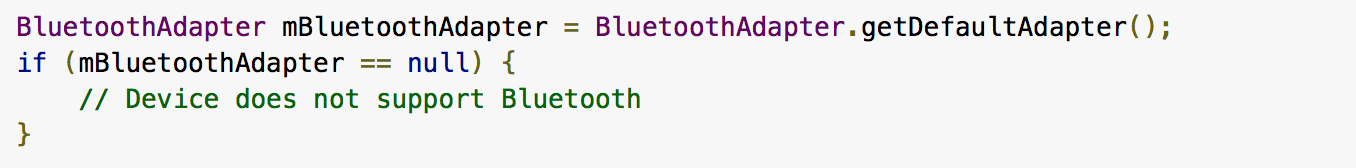
\includegraphics[scale=0.60]{bluetooth_enabled}
  	\caption{Trecho de código exemplificando a comunicação \textit{bluetooth}}
  	\label{img:bluetooth_enabled}
  	\end{figure}
  	
  	Para garantir que o dispositivo \textit{bluetooth} será adicionado apenas uma vez, será utilzado um trecho de código parecido com o da figura \ref{img:bluetooth_devices}, que garante que para um dispositivo ser adicionado ele, não deve estar presente na lista de dispositivos previamente adicionados.
  	
  	\graphicspath{{figuras/}}
  	\begin{figure}[h]
  	\centering
  	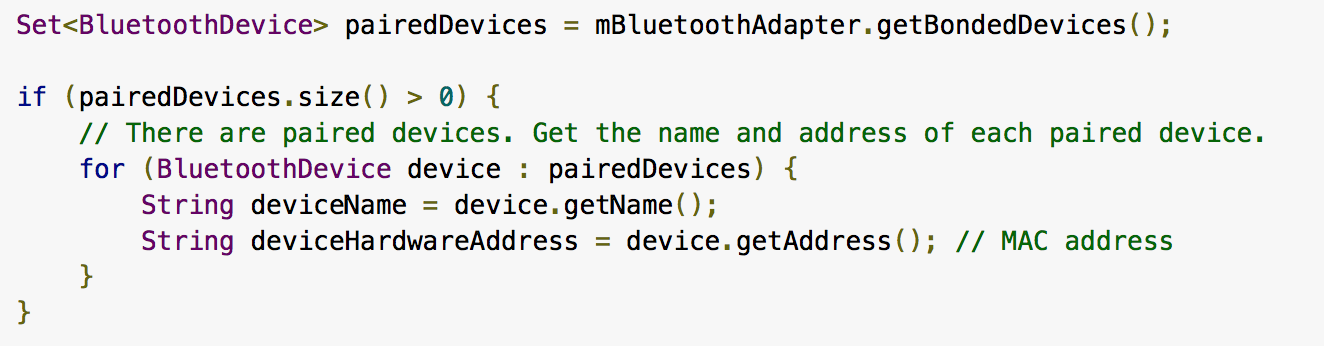
\includegraphics[scale=0.60]{bluetooth_paired_devices}
  	\caption{Trecho de Código que garante que um dispositivo será adicionado apenas uma vez}
  	\label{img:bluetooth_devices}
  	\end{figure}
  	
  	Para que seja feita a transferência de dados entre os dispositivos, o Google (empresa responsável pela documentação da plataforma android), dispõe um trecho de código que serve como guia para implementação desta funcionalidade. Na figura \ref{img:trecho1} é criada uma classe que define as constantes que serão utilizadas ao longo do código.
  	
  	\graphicspath{{figuras/}}
  	\begin{figure}[h!]
  	\centering
  	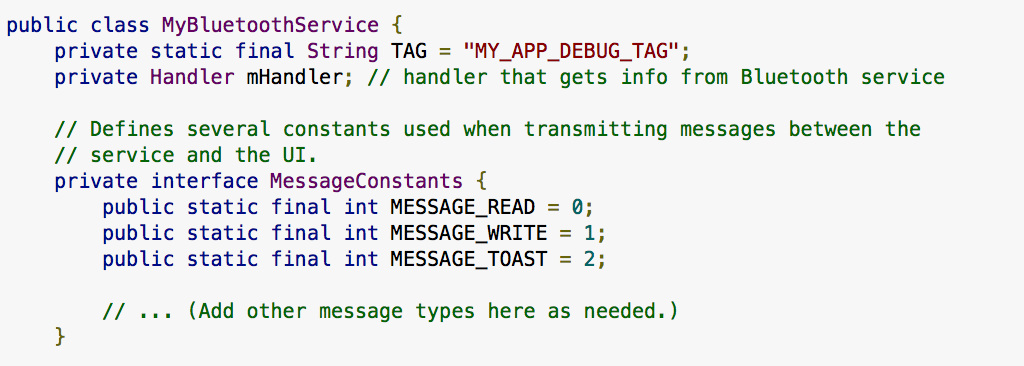
\includegraphics[scale=0.60]{classe_MyBluetoothService}
  	\caption{Neste trecho de código são definidas as constantes que serão utilizadas ao longo do código}
  	\label{img:trecho1}
  	\end{figure}
  
Na figura \ref{img:trecho2} é criada uma outra classe que é a classe que implementa a funcionalidade de troca de dados. Esta classe extende da classe Thread, seus atributos são do tipo \textit{BluetoothSocket}, \textit{InputStream}, \textit{OutputStream} e um \textit{array} de \textit{byte}.

\graphicspath{{figuras/}}
\begin{figure}[h!]
\centering
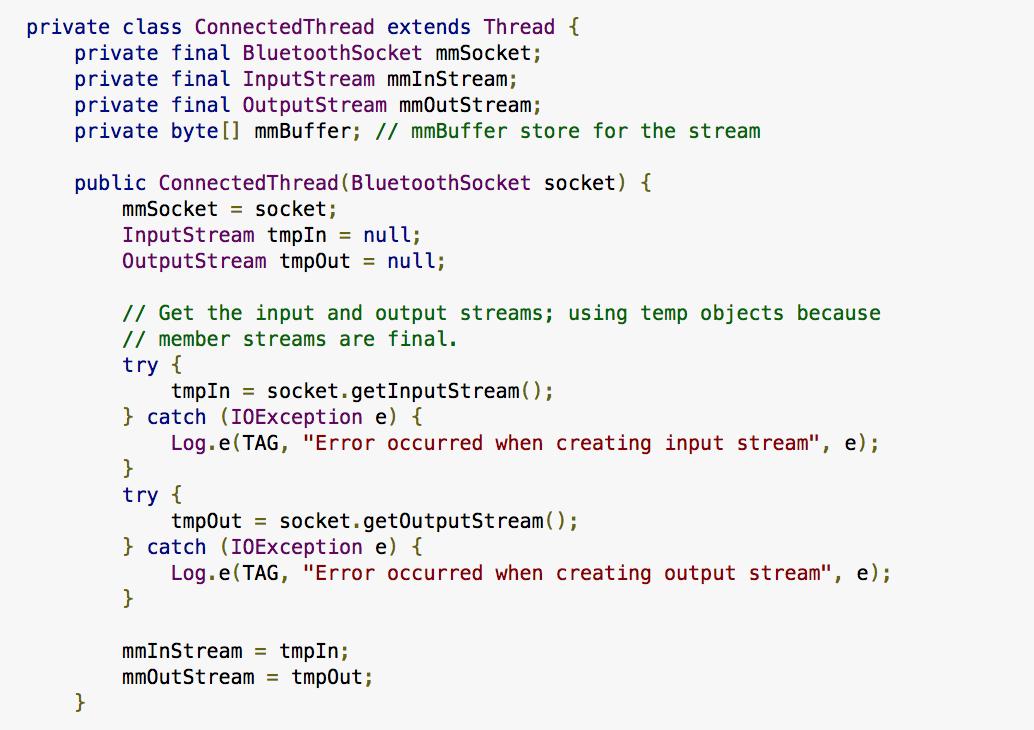
\includegraphics[scale=0.80]{classe_ConnectedThread}
\caption{Nesta classe são implementados os métodos responsáveis pelo funcionamento da troca de dados}
\label{img:trecho2}
\end{figure}

A figura \ref{img:trecho3} apresenta o método \textit{"run"} que funciona em segundo plano constantemente. Este método é responsável por ficar aguardando uma requisição do dispositivo.

\graphicspath{{figuras/}}
\begin{figure}[h!]
\centering
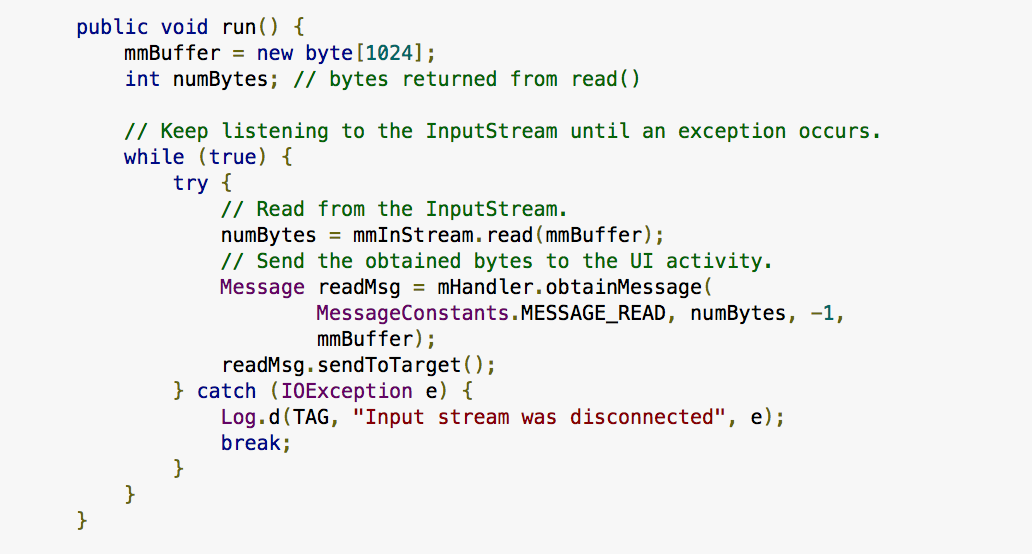
\includegraphics[scale=0.80]{run_method}
\caption{Implementação do método \textit{run} que é responsável por receber as informações do dispositivo \textit{bluetooth}}
\label{img:trecho3}
\end{figure}

O método \textit{"write"} é que faz a escrita dos dados que serão enviados para o dispositivo, como pode ser visto na figura \ref{img:trecho4}.

\graphicspath{{figuras/}}
\begin{figure}[h]
\centering
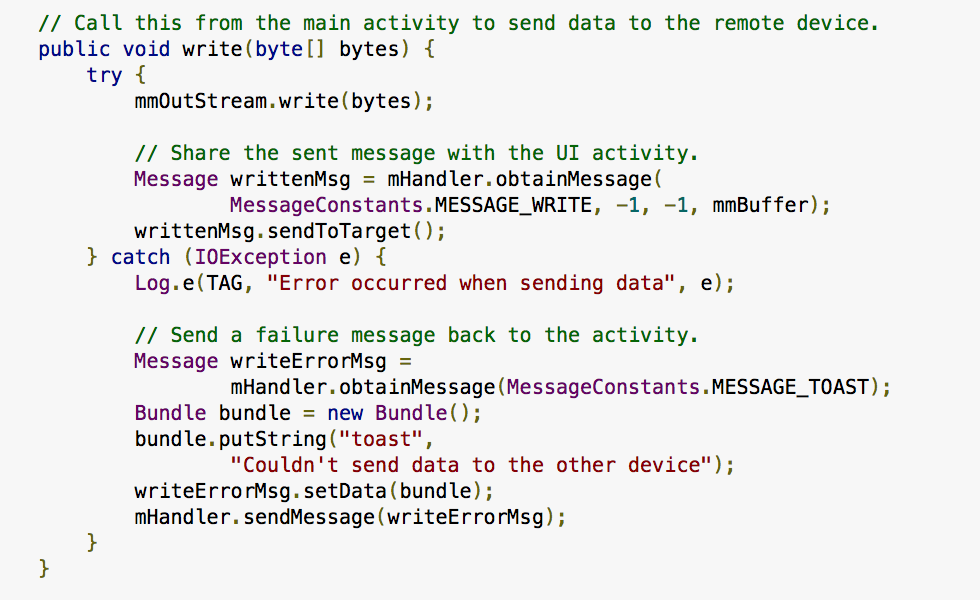
\includegraphics[scale=0.80]{write_method}
\caption{Implementação do método \textit{write} que é responsável por escrever os dados que serão enviados}
\label{img:trecho4}
\end{figure}

Por último, o método \textit{"cancel"} que encerra a conexão com o dispositivo pareado, como mostrado na figura \ref{img:trecho5}

\graphicspath{{figuras/}}
  \begin{figure}[h]
  \centering
  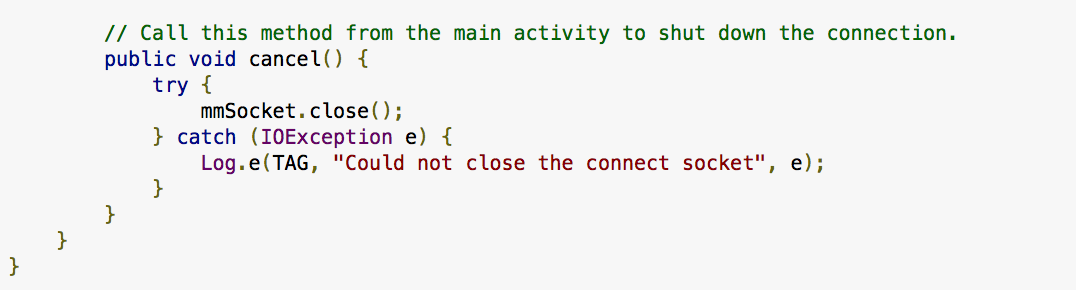
\includegraphics[scale=0.80]{cancel_method}
  \caption{Método \textit{"cancel"} que encerra a conexão com o dispositivo}
  \label{img:trecho5}
  \end{figure}  
  
  \section{Eletroeletrônica}
  
  \section{Alimentação}
  
  \section{Estrutura}
  
  \section{Normas}
  